\chapter{Aspectos Generales}
\section{Aspectos Generales}
\subsection{Descripción del Problema}
Uno de los sentidos más importantes de los seres humanos es la visión. Ésta es empleada para obtener la información visual del entorno físico. Según Aristóteles, “Visión es saber que hay y donde mediante la vista”. De hecho, se calcula que más del 75\% de las tareas del cerebro son empleadas en el análisis de la información visual. El refrán popular de “Una imagen vale más que mil palabras” tiene mucho que ver con los aspectos cognitivos de la especie humana. Casi todas las disciplinas científicas emplean utillajes gráficos para transmitir conocimiento\footnote[1]{Visión Humana, fuente: Sistemas Adaptativos y Bioinspirados en Inteligencia Artificial\href{http://sabia.tic.udc.es/}{(S.A.B.I.A.)}}.

Uno de los más grandes concursos a nivel mundial en clasificación de imágenes reporta que las técnicas tradicionales (como las técnicas de extracción de características en imágenes estáticas: \textit{Principal component analysis} (PCA), \textit{Edges detector}, \textit{Gabor waveled}; Video: PCA, \textit{Discrete cosine transform} (DCT), \textit{optical flow} e \textit{image difference}) están siendo superadas por técnicas de \textit{Deep Learning} basadas en el proceso cerebral humano. Dicho éxito se debe a que las técnicas tradiciones requieren de un ambiente controlado y no son tolerables a cambios como: traslación, rotación y escalado, por otro lado las técnicas de \textit{Deep Learning} demustran ser mas robustas y efectivas frente a estos tipos de cambios\footnote[2]{\textit{Deep Learning} vs. \textit{Machine Learning} fuente: \href{http://www.image-net.org/}{Analytics Vidhya}}.
	
Diversas actividades cotidianas necesitan del reconocimiento de imágenes, tal es el caso del reconocimiento de expresiones faciales, que en los últimos años se ha convertido en una de las tareas más estudiadas por investigadores en todo el mundo, con el fin de alcanzar un margen de error minimo para posteriormente centrarse en el desarrollo de aplicaciones en distintos campos, como: estudio de marketing, interacción hombre-máquina, psicología y análisis educativo \footnote[3]{Las expresiones faciales de las emociones, historia y aplicaciones, fuente: \href{http://medina-psicologia.ugr.es/cienciacognitiva/?p=664}{Ciencia Cognitiva}}, las cuales han sido abordada por diferentes técnicas tradicionales no obteniendo los resultados prometedores en imagenes reales que contienen distintos tipos de variaciones (mencionados en el parrafo anterior) limitando asi la implementacion y desarrollo de aplicaciones utiles para el bien comun (aplicaciones antes mencionadas).

\subsection{Identificación del Problema}
Las técnicas tradicionales para el reconocimiento de expresiones faciales usadas en la actualidad necesitan de un ambiente controlado (iluminacion constante, alta calidad de imagen, poco ruido, imagen sin oclusión), y no son tolerables a cambios como rotación, traslación, escalado, limitando asi la creacion de aplicaciones con imagenes del mundo real(imagenes obtenidas a partir de camaras de seguridad) . Por lo que hay la necesidad de usar nuevas técnicas del estado del arte que nos permitiran obtener mejores resultados superando asi la limitacion antes mencionada.

\section{Antecedentes}
Se muestra una lista de trabajos resaltantes que hacen uso de tecnicas de \textit{Deep Learning}, los cuales sirvieron de inspiración y fuente de información valiosa en el desarrollo de este trabajo. Tambien se presentan trabajos dedicados al reconocimiento de expresiones faciales utilizando tecnicas tradicionales de vision por computador y \textit{machine learning}.

\vspace{1cm}
\textbf{“Image based Static Facial Expression Recognition with Multiple Deep Network Learning” \cite{yu2015image}}\\
%\textbf{Descripción:}\\

\begin{itemize}
\item En este trabajo, es propuesto un detector de rostros y un clasificador de expresiones faciales en imagenes.
\item Para la deteccion de rostros en las imagenes, es usado un conjunto de tres detectores de rostros del estado del arte. 
\item Para el reconocimiento de las expresiones faciales, es creado un clasificador basado en un conjunto de 
Redes Neuronales Convolucionales(CNNs).
\item El modelo creado es evaluado en en la base de datos publico SFEW 2.0, logrando resultados del estado del arte.
\item Los resultados obtenidos en este trabajo
son 55.96 \% y 61.29 \% en el conjunto de datos de validacion y test respectivamente de la base de datos SFEW 2.0.
\end{itemize}

\textbf{“A Facial Expression Recognition System Using
Convolutional Networks” \cite{lopes2015facial}}\\

\begin{itemize}
\item En este trabajo, los autores proponen combinar metodos de pre-procesamiento de imagenes y Redes Neuronales Convolucionales para el reconocimiento de expresiones faciales.
\item En el paso de pre-procesamiento  las imagenes de entrada son normalizados espacialmente. asi tambien, la intensidad de los pixels son normalizados y como ultimo es recortada la region de la imagen que contiene solo el rostro humano.
\item Para reconocer las expresiones faciales es usado una arquitectura de Red Neural Convolucional.
\item  Prueban que las operaciones de pre-procesamiento tienen un impacto directo en el rendimiento del clasificador CNN.

\item Para la creacion del clasificador hacen uso de una GPU de 1.5GB.
\item Este trabajo es evaluado en la base de datos CK+.

\item Los resultados obtenidos alcanzan un nivel de precision del 97.81 \% .
 
\end{itemize}



\textbf{“A Real-time Facial Expression Recognizer using Deep
Neural Network” \cite{jeon2016real}}\\

\begin{itemize}
\item En este trabajo, es propuesto un  clasificador de expresiones faciales en tiempo real.
\item Primero, es detectado el rostro humano en las imagenes usando \textit{HOG feature descriptor}.
\item Segundo, es usado un metodo para el seguimiento del rostro basado en un rastreador de correlación.
\item Por último, es reconocido la expresion facial usando un modelo de Red Neuronal Convolucional.
\item Para la creacion del clasificador usan una GPU con 768 cores.
\item El modelo propuesto en este trabajo es evaluado en base de datos publico FER2013.
\item Los resultados obtenidos por el  modelo en la base de datos FER2013  alcanzan un nivel de precision de  70.74\%
\item Adicionalmente, el modelo evalua 9.1 fps.
\end{itemize}



\textbf{“Real-time Personalized Facial Expression
Recognition System
Based on Deep Learning” \cite{lee2016real}}\\

\begin{itemize}
\item En este trabajo, es propuesto un clasificador de expresiones faciales en tiempo real usando una camara web en un sistema personalizado que contiene personas identificadas por un ID.
\item El modelo propuesto logra detectar y reconocer expresiones faciales de personas a una distancia de 2~3m en un entorno para  television.
\item Un modelo CNN inicial es entrenado usando la base de datos FER2013.
\item Los pesos obtenidos en la fase de entrenamiento del modelo inicial son usados para la inicializacion del modelo CNN personalizada.
\item Un conjunto de 200 imagenes por persona identificada en el sistema es recolectado.
\item Por medio de transformaciones del conjunto imagenes de cada persona identificada en el sistema es obtenido un total de 2400 imagenes por persona.
\item La CNN personalizada es entrenada en el conjunto de imagenes por persona que fue obtenida por medio de las transformaciones.
\item El modelo CNN personalizada logra un resultado del 96 \% de precision a una distancia de 3m en el conjunto de personas identificadas en el sistema.

\end{itemize}


\section{Objetivos}
\subsection{Objetivo General}
Desarrollar una arquitectura de Red Neuronal Convolucional que sea capaz de obtener niveles de precision confiables (con un minimo margen de error) en el reconocimiento de expresiones faciales, permitiendo asi contribuir en el desarrollo de futuras aplicaciones del mundo real que sirvan para el beneficio de la sociedad.
\subsection{Objetivos Específicos}
\begin{itemize}
\item Selección de las bases de datos de expresiones faciales y transformación de datos a un formato estandar para su posterior utilizacion.
\item Investigar los filtros de convolucion para la correcta seleccion de los parametros.
\item Investigar la funcion de submuestreo para la correcta selección de los parametros. 
\item Investigar las funciones de activación y funciones de normalizacion para la correcta selección de los parametros.
\item Diseñar la arquitectura propuesta(configuracion de parametros, numero de capas y funciones de activacion y normalizacion), basandonos en los objetivos previos.
\item Entrenar la arquitectura propuesta.	
\item Evaluar el modelo creado a partir de la arquitectura propuesta.
\item Analizar e interpretar los resultados
\end{itemize}

\section{Alcances}
En este trabajo de investigacion se lograron los siguientes alcances.

\begin{itemize}
\item Se propuso una nueva arquitectura para el reconocimiento de expresiones faciales, basada en las Redes Neuronal Convolucional, capaz de obtener altos niveles de precision que seran de utilidad para el desarrollo de futuras aplicaciones del mundo real.
\item Se creo una nueva base de datos, la cual fue resultado de la union de las dos bases de datos antes mencionadas(FER2013 y CK+).
\item Contribuimos con la comunidad academica del país y la region brindandoles informacion de un tema de investigación actual que servira como base para el desarrollo de futuras aplicaciones y trabajos relacionados.
\end{itemize}
 

\section{Justificación}
En la actualidad se ha dado más realce a algunas disciplinas de la inteligencia artificial como: \textit{Machine Learning} y \textit{Deep Learning}, disciplinas que brindan distintas técnicas que están dando solución a problemas de clasificación de imágenes, comprensión de escena, análisis de sentimientos y otros. Así es el caso de la visión artificial donde las Redes Neuronales Convolucionales está proporcionando mejores resultados en comparación con algoritmos y técnicas tradicionales.

En este trabajo, presentamos un estudio resumido de la investigación hecha en \textit{Deep Learning} que servirá tanto para los investigadores como para los lectores. También este trabajo ayudara para el desarrollo de futuros proyectos de clasificación de imágenes en distintos campos (seguridad, medicina y biología, internet y la nube, entretenimiento, maquinas autónomas y otros)\footnote[4]{Aplicaciones de Deep Learning, fuente: \href{https://developer.nvidia.com/deep-learning}{NVIDIA} GPUs - el motor del aprendizaje profundo(deep learning)}.


\section{Metodología}
Dada la naturaleza del trabajo de investigación, se utilizó los métodos de investigación bibliográfica, explorativa y aplicativa. Bibliográfica ya que se recogió y analizo información para obtener conocimientos previos sobre \textit{Deep Learning} y el detector \textit{Haar Cascade}. Explorativa porque se seleccionó información relevante procedente de la etapa de investigación bibliográfica, para la construcción de la arquitectura de una Red Neuronal Convolucional basándonos en trabajos previos relacionados con la línea de investigación. Aplicativa por que se utilizaron los conocimientos adquiridos \cite{19sabino1994hacer}\cite{23silva2001metodologia}.


\section{Limitaciones}
\begin{itemize}
\item Dificil acceso a herramientas tecnológicas de hardware, principalmente GPU's de alta capacidad, necesarias para la fase de entrenamiento de la Red Neuronal Convolucional. Por consiguiente, la solución es alquilar servidores en la nube especializados en el entrenamiento de arquitecturas de \textit{Deep Learning}.
\item Carencia de organizaciones peruanas que brinden bases de datos para poder utilizarlos en la fase de entrenamiento ya que se requiere miles de imágenes (imágenes de acuerdo al proyecto de investigación en el que se trabaje, como: rostros, danzas, señas, sitios arqueológicos y entre otros) para que se cree un modelo eficiente y robusto, llevando a utilizar base de datos de organizaciones extranjeras que fomentan la investigación en esta área.
\end{itemize}
\newpage
\section{Cronograma de Actividades}
\begin{table}[!htb]
    \centering
    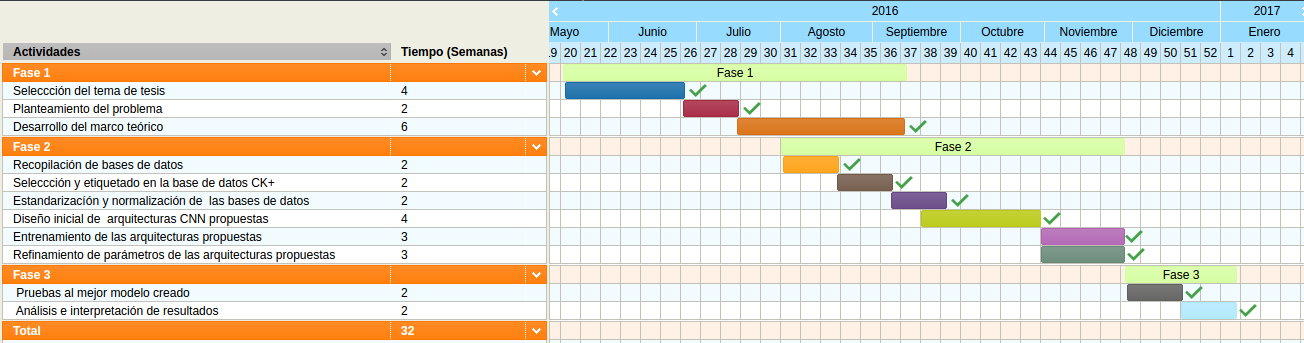
\includegraphics[angle=90,width=60mm]{Imagenes/cronograma.png}
    \caption{Cronograma de actividades}
    \label{tab:tab1}
\end{table}


